\section{Method}\label{sec:method}

The goal of \NAME{} (\cref{fig:fig2}) is to enhance objects' signal by isolating and emphasizing their motion in video with a non-stationary, fluid background. Inspired by prior work \cite{sun2022bkind, jakab2018conditionalImageGen, ryou2021weaksupKPdisco}, we use an encoder-decoder framework. Our contribution is twofold: (1) a reconstruction target based on spatiotemporal differences across neighboring frames, and (2) a denoising metric that does not require clean ground truth. The method assumes that background spatiotemporal statistics differ from those of the foreground. 
% We also rely on objects-of-interest to sparsely fill the frame and to have higher pixel-intensity values than background.

\subsection{Self-supervised denoising}
In our benchmarks' low-SNR videos, signals are distributed across time; as such, we want to condense information from multiple timesteps into a single frame to exaggerate the signal. We do this through the reconstruction target. For simplicity, we choose to reconstruct the spatiotemporal combination of 3 frames, expressed, in \cref{eqn:reconstruction_target}, from three input frames, $I_t$, $I_{t-T}$, and $I_{t-2T}$. We explore a vanilla autoencoder, UNets with and without skip connections and residual layers, and 3D convolutions (in \cref{tab:big_table}), and find a simple encoder-bottleneck-decoder framework optimal. We also explore $N>3$ input frames, $T>1$, the target without the DAE network as input to downstream tasks, and more in our ablations in the Supplemental \cref{tab:ablation_reconstruction_targets}, \ref{tab:additional_ablations}, and \cref{fig:reconstruction_targets_supp}. 

% Given a noisy video, our method aims to reconstruct a combination of the input frame at time $t$, $I_t$, and the spatiotemporal differences with a previous frame at time $t-T$ and a future frame at time $t+T$. 
% Unlike many denoising methods, which rely on removing motion blur and/or speckle to boost the signal to noise ratio, our method relies on convolutions withing a neural network to remove the noise, while simultaneously augmenting the target object to boost the signal. 
We use an encoder-decoder architecture, seen in \cref{fig:fig2}, with a spatial encoder, $\Phi$, a temporal hourglass network, $\Theta$, and a reconstruction decoder, $\Psi$. During training, spatial encoders, $\Phi$, take $I_t$, $I_{t-T}$, and $I_{t-2T}$ as input to generate spatial feature embeddings, which are then used by the hourglass network, $\Theta$, to generate a spatiotemporal feature embedding; this embedding passes to $\Psi$ to reconstruct the learning objective $\hat{S}_{t,T}$.
% Pietro: the signal is distributed across multiple frames, so the ideal detector would be one that acts across multiple frames at a time, in this case we kept using the frame-by-frame detectors for which there is a vast literature, and we wanted to summarize the temporal information from past and future into one frame in which detection happens 
% the way to motivate is is we want to use off-the-shelf frame-by-frame detectors and we want to summarize the past, present and future into one window; for this paper, for simplicity we wanted to focus on 3 frames; in the future we could experiment with more
% P future work: hypothesizing many different velocities, testing them out, and then getting the one with the highest contract
\begin{equation}
\hat{S}_{t,T}=\Psi(\Theta(\text{concat}(\Phi(I_t), \Phi(I_{t-T}), \Phi(I_{t-2T}))))
\end{equation}
% All three components are jointly trained.
% \SUZ{Wording?} with one single reconstruction loss backpropagated through each component. 
% The high-level architecture can be seen in \cref{fig:fig2}; more detail is in the Supplemental Materials \cref{tab:architecture}.

\subsection{Reconstruction target and loss}\label{sec:reconstruction}

\textbf{Target.} 
% We experimented with several possible reconstruction targets, as seen in \cref{tab:ablation_reconstruction_targets} and \cref{fig:reconstruction_targets_supp}. Ultimately, w
We use the \textit{directionally-positive frame difference with the current frame (PFDwTN)} as our reconstruction target. This combines the current frame with the positive motion from the previous and next frames. Directionally-positive motion of the next frame is defined: $\max(0, I_{t+T} - I_t)$; of the previous frame, it is defined: $\max(0, I_{t-T} - I_t)$. In both cases, motion is relative to the current frame $I_t$. Note that the previous frame $I_{t-T}$ goes into the network, while the future frame $I_{t+T}$ does \textit{not}. It is used only when calculating the ground-truth target for the loss.
 
\looseness-1 
To handle frames where the background movement does not differ significantly from the foreground objects' motion (\ie, stationary objects), we include the original frame, $I_t$, in the reconstruction target. The overall target is:
\begin{equation}\label{eqn:reconstruction_target}
S_{t,T} = \max(0, I_{t-T} - I_t) + I_t + \max(0, I_{t+T} - I_t)
\end{equation}

Other motion-augmenting targets that we tested are defined/visualized in Sec. \ref{sec:ablation_additions} and \cref{fig:reconstruction_targets_supp} in the Supp. Mat.

\noindent{}\textbf{Loss}. We apply mean-squared-error loss for reconstructing the current frame with augmented motion signatures:
\begin{equation}\label{eqn:recon_loss}
\mathcal{L}_{recon} = \|\hat{S}_{t,T}-S_{t,T}\|_2
\end{equation}



\subsection{Noise Removal Network}\label{sec:method_arch}

\noindent{}\textbf{Appearance Encoder $\Phi$}. We implement a 6-layer CNN. Each layer consists of a convolutional block (Conv2D + ReLU) followed by max pooling, progressively increasing the number of feature channels while reducing the spatial dimension, $\mathbb R^{(H,W,1)} \rightarrow \mathbb R^{(\frac{H}{32},\frac{W}{32}, 512)}$. We also save skip connections (sequential max pools and 1x1 convolutions) to be used by the hourglass network and decoder. This design uses a fraction of the parameters and FLOPs from an off-the-shelf UNet, to let the network capture multi-scale features efficiently. See \cref{tab:denoiser_time} for efficiency comparisons.

\noindent{}\textbf{Temporal Hourglass Network $\Theta$} is an hourglass network with a bottleneck consisting of two 3x3 convolutional layers with 512 channels, each followed by ReLU activation. We also have skip connections as feature combiners at each level of the network, designed to merge information from the provided appearance features' skip connections.

\noindent{}\textbf{Reconstruction Decoder $\psi$} has 6 upsampling stages, each consisting of a ConvTranspose followed by convolutions and ReLU activations. At each layer, the skip connections from the corresponding encoder level are concatenated with the upsampled features. The decoder reduces the number of channels while increasing the spatial dimension ending with a single-channel output, $\mathbb R^{(\frac{H}{32},\frac{W}{32}, 512)} \rightarrow \mathbb R^{(H,W,1)}$.

More details on each of these modules is in the Supplemental materials \cref{tab:denoiser_arch}.

% \subsection{Noise removal}

\subsection{Denoising Metric}\label{sec:denoising_metric}
Typically \cite{krull2019noise2void, laine2019high, jang2023selfsupervised, huang2021neighbor2neighbor, Sheth_2021_ICCV}, denoising networks use Peak Signal-to-Noise Ratio (PSNR) and Structural Similarity Index Measure (SSIM) \cite{wang2004ssim} as evaluation metrics. PSNR is the ratio of maximum signal power to noise power, and SSIM measures perceived image quality. Both metrics rely on having clean imagery for comparison. Our denoising approach is unsupervised -- we do \textit{not} have clean imagery. As a result, we design a new metric, Foreground-to-Background Divergence ($FBD$), to evaluate denoised performance when we have detection annotations, and we rely on downstream performance as a proxy for denoised performance on datasets with different task annotations.

\subsubsection{Foreground-to-Background Divergence (\textit{FBD}) Metric for Unsupervised Denoising} \label{sec:KL} 
Recall that we assume that our \textit{downstream} models are supervised. Therefore, for detection tasks, we can assume we have bounding boxes or segmentation masks. For simplicity, we call detection annotations ``boxes'', though the same approach works for segmentation masks. 

$FBD$ measures how well a denoising method makes objects distinguishable from background by computing the KL-Divergence between a region containing an object (foreground) and the same region at a different time without it (background). An example is shown in \cref{fig:fbd_example}. Unlike PSNR, which requires a clean reference, $FBD$ does not, which is critical in many real-world applications.

\begin{figure}
    \centering
    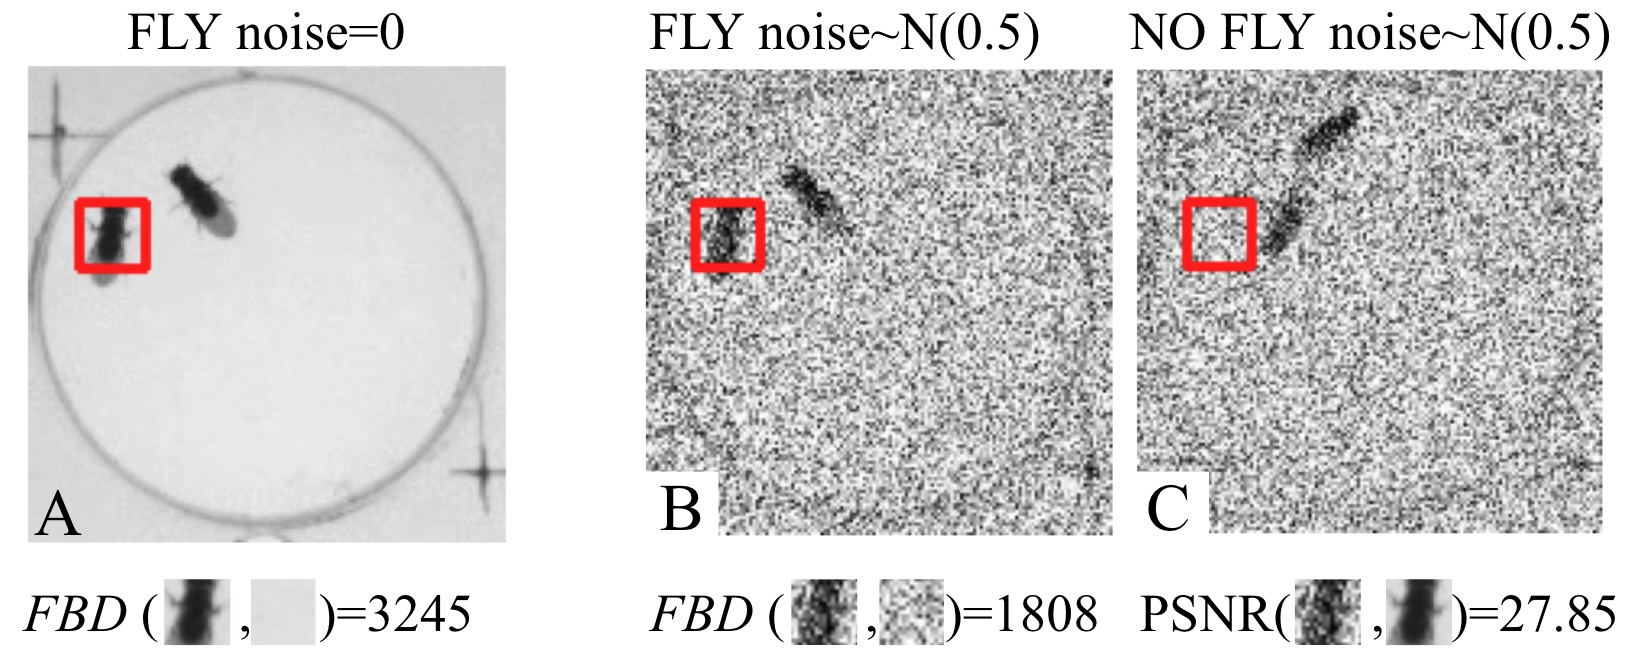
\includegraphics[width=0.5\textwidth]{figs/FBD_no_B.jpg}
    \caption{High-SNR visualization and calculations for $FBD$ and PSNR on Fly-vs-Fly \cite{flyvfly} with synthetic noise. In order to calculate the PSNR of \textbf{(B)}, a `clean' image \textbf{(A)} is needed. \textbf{(A)} is not needed for $FBD$, though \textbf{(C)} is.\vspace{-2mm}}
    \label{fig:fbd_example}
\end{figure}

For each object's box $b$ in each frame $I$ of each video, we take the density of pixel intensity values: $d_{b} = I[b]$, where $b$ are the indices associated with the box. Then, we take the density of pixel intensity values from a different frame $\tilde{I}$ of the \textit{same} video at the same box location $b$ where we know there is no object, $\tilde{d}_b$. If the distributions are separable \ie, the distribution of object pixels is distinct from the distribution of background pixels, then the denoising method works as intended. We measure the separability between object and non-object via the Kullback-Leibler (KL) Divergence \cite{Kullback51klDivergence}. KL divergence measures the distance between two probability distributions P and Q as follows:
\begin{equation}
D_{KL}(P\|Q) = \int p(x) \log(\frac{p(x)}{q(x)}) dx
\end{equation}
To generate a metric for a data split, we average the $D_{KL}$ over all N bounding boxes to get 
\begin{equation}\label{eqn:fbd}
FBD_{D_{KL}} = \frac{1}{N}\sum_{b\in{N}} D_{KL}( d_b \|\tilde{d}_b)
\end{equation}
A visualization of this metric can be seen in Supplementary materials  Fig.\ \ref{fig:denoiser_metric_details}. A larger score (divergence) indicates greater distinguishability of objects from background.